\documentclass[french]{article}
\usepackage[T1]{fontenc}
\usepackage[utf8]{inputenc}
\usepackage[french]{babel}
\usepackage{amsmath}
\usepackage{mathtools}
\usepackage{color}
\usepackage[svgnames,dvipsnames]{xcolor} 
\usepackage{soul}
\usepackage{amssymb}
\usepackage{enumitem}
\usepackage{multicol}
\usepackage[left=2cm,right=2cm,top=2cm,bottom=2cm]{geometry}
\newcommand{\mathcolorbox}[2]{\colorbox{#1}{$\displaystyle #2$}}
\usepackage{pifont}
\usepackage{pst-all}
\usepackage{pstricks}
\usepackage{delarray}
\usepackage{setspace}
\usepackage{graphicx}
\usepackage{hyperref}
\usepackage{nicematrix}

\hypersetup{
	colorlinks=true,
	linkcolor=blue,
	filecolor=magenta,      
	urlcolor=cyan,
	pdftitle={Overleaf Example},
	pdfpagemode=FullScreen,
}

\usepackage{amsthm}
\newtheorem*{Rem}{Remarque}

\begin{document}
	LECOURTIER Frédérique \hfill \today
	\begin{center}
		\Large\textbf{{Suivi Stage PhiFEM : 06/02/2023 - 28/07/2023}}\\
	\end{center}
	\tableofcontents
	\newpage
	
	\section{Semaine 1 : 06/02/2023 - 10/02/2023}
\graphicspath{{semaines/semaine_1/images/}}

\begin{abstract}
	Pendant cette première semaine, j'ai du me familiariser avec le code "phifem" écrit par Vincent Vigon et les codes de génération des données fournit par Killian. L'idée étant de comprendre comment générer les données avec FEniCS pour ensuite les faire apprendre par un FNO. Après la réunion du 07/02, il semblerait que le sujet du stage porte sur l'entrainement d'un FNO puis la correction/certification des prédictions.
\end{abstract}

\subsection{Génération des données}

Le code fournit par Killian (\href{https://colab.research.google.com/drive/1AJr5JaNs_gnbJce7zE2rfbjicwPxjdtL}{"Data\_Generation\_moving\_ellipse\_poisson"}) a pour but de faire varier la levelset. J'ai donc repris ce code afin de générer dans un premier temps les données solution d'un problème de Poisson avec condition de Dirichlet homogène (\href{https://colab.research.google.com/drive/1dHHFmfDs9XiMoT5EMKXQ1OFFKB3138c2}{"DataGen\_PhiFEM\_f\_gaussienne"}). 

On considère $\Omega$ le cercle de rayon $\sqrt{2}/4$ et de centre $(0.5,0.5)$ avec $\Phi(x,y)=-1/8+(x-1/2)^2+(y-1/2)^2$ et le domaine fictif $O=(0,1)^2$.

On souhaite résoudre 
\begin{equation*}
	\begin{cases}
		-\Delta u &= f\,, \quad \text{dans $\Omega$}\,, \\
		u &= 0\,, \quad \text{sur $\Gamma$}\,, \\
	\end{cases}
\end{equation*}
où 
$$f(x,y) = \exp\left(-\frac{(x-\mu_0)^2 + (y-\mu_1)^2}{2\sigma^2}\right)\,, $$ 
avec $\sigma \sim \mathcal{U}([0.1,0.6])$ et $\mu_0, \mu_1 \sim \mathcal{U}([0.5-\sqrt{2}/4, 0.5+\sqrt{2}/4])$ à condition que $\phi(\mu_0, \mu_1) < -0.05$. 

\begin{minipage}{0.48\linewidth}
	\centering
	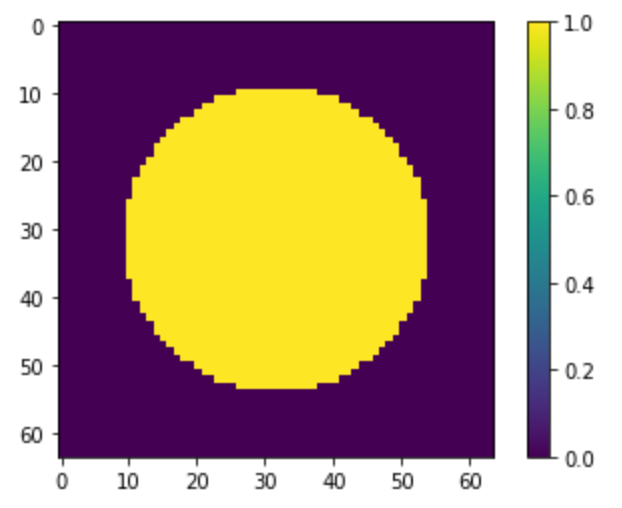
\includegraphics[width=0.5\linewidth]{domaine.png}
\end{minipage}
\begin{minipage}{0.48\linewidth}
	\centering
	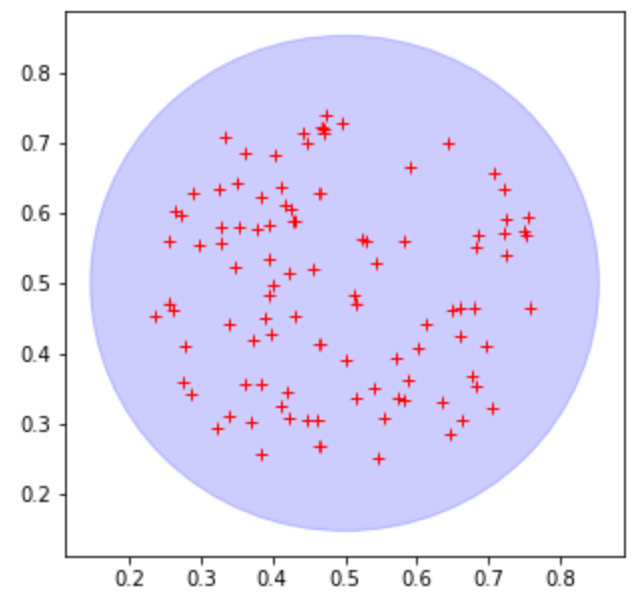
\includegraphics[width=0.45\linewidth]{parametres.png}
\end{minipage}

La fonction \textit{create\_data} renvoie le nombre donné de $F$ et les paramètres associés choisis uniformément. 

\textbf{Formulation faible :}
$$\int_{\Omega_h}\nabla(\bar{\phi}w)\nabla(\bar{\phi}v)-\int_{\partial\Omega_h}\frac{\partial}{\partial n}(\bar{\phi}w)\bar{\phi}v+G_h(w,v)=\int_{\Omega_h}f\bar{\phi}v+G_h^{rhs}(v)$$
avec
$$G_h(w,v)=\sigma h\sum_{E\in\mathcal{F}_h^\Gamma}\int_E\left[\frac{\partial}{\partial n}(\bar{\phi}w)\right]\left[\frac{\partial}{\partial n}(\bar{\phi}v)\right]+\sigma h^2\sum_{T\in\mathcal{T}_h^\Gamma}\int_T \Delta(\bar{\phi}w)\Delta(\bar{\phi}v)$$
et
$$G_h^{rhs}(v)=-\sigma h^2\sum_{T\in\mathcal{T}_h^\Gamma}\int_T f\Delta(\bar{\phi}v)$$

On utilise \href{https://fenicsproject.org/}{FEniCS} (solveur d'EDP) pour résoudre le problème. 

On va finalement stocker les résultats au format npy dans les fichiers "F.npy", "agentParams.npy" et "U.npy"

\newpage

\subsection{FNO}

De la même manière que pour la génération des données, il a fallu reprendre le code de Vincent Vigon (\href{https://colab.research.google.com/drive/1dOIb8N1i6FWXZPOvuP8xFIxmf0kjQysR}{"phifem"}) afin de l'adapter au problème considéré (\href{https://colab.research.google.com/drive/1-OdXA3xj5_X-xwvYplRStopU1yQe7AOg}{phifem\_f\_gaussienne}). 

Une première étape fut donc la lecture d'article sur les FNO (Fourier Neural Operator). Voici un schéma descriptif de ce type de réseau de neurones. 

\begin{minipage}{\linewidth}
	\centering
	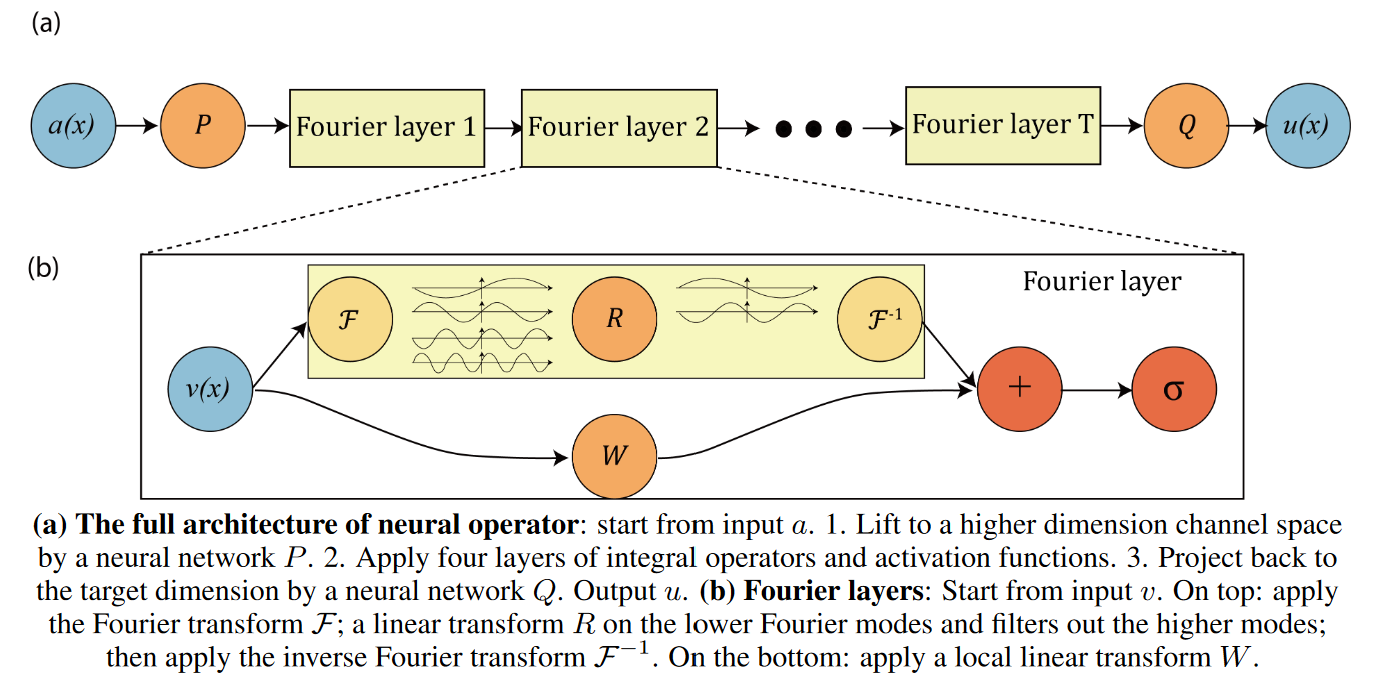
\includegraphics[width=0.7\linewidth]{FNO.png}
\end{minipage}

L'idée étant que le réseau nous retourne $u$.

\begin{Rem}
	ERREUR : il doit nous retourner $w$ car on connait déjà la levelset et pour la correction, ça n'a pas de sens de faire $\phi u=\phi^2 w$.
\end{Rem}

\subsection{Correction}

On veut en fait résoudre le même problème sauf que cette fois-ci, on définit une nouvelle levelset $\bar{\phi}=\phi u$ (où $u$ est la sortie du FNO).

On résout alors le nouveau problème $z=\bar{\phi}C$ :
\begin{equation*}
	\begin{cases}
		-\Delta z &= f\,, \quad \text{dans $\Omega$}\,, \\
		z &= 0\,, \quad \text{sur $\Gamma$}\,, \\
	\end{cases}
\end{equation*}

\begin{Rem}
	L'idée étant d'appliquer la correction sur un millage plus grossier que le réseau. Ainsi FNO+Corr plus précis que Phifem classique et plus rapide.
\end{Rem}

Les résultats obtenus (en prenant ici $u_{ex}=cos\left(\frac{\pi}{2}\times\left(\frac{4}{\sqrt{2}}\right)^2\times\left((x-0.5)^2+(y-0.5)^2\right)\right)$) ne sont pas bons :

\begin{minipage}{\linewidth}
	\centering
	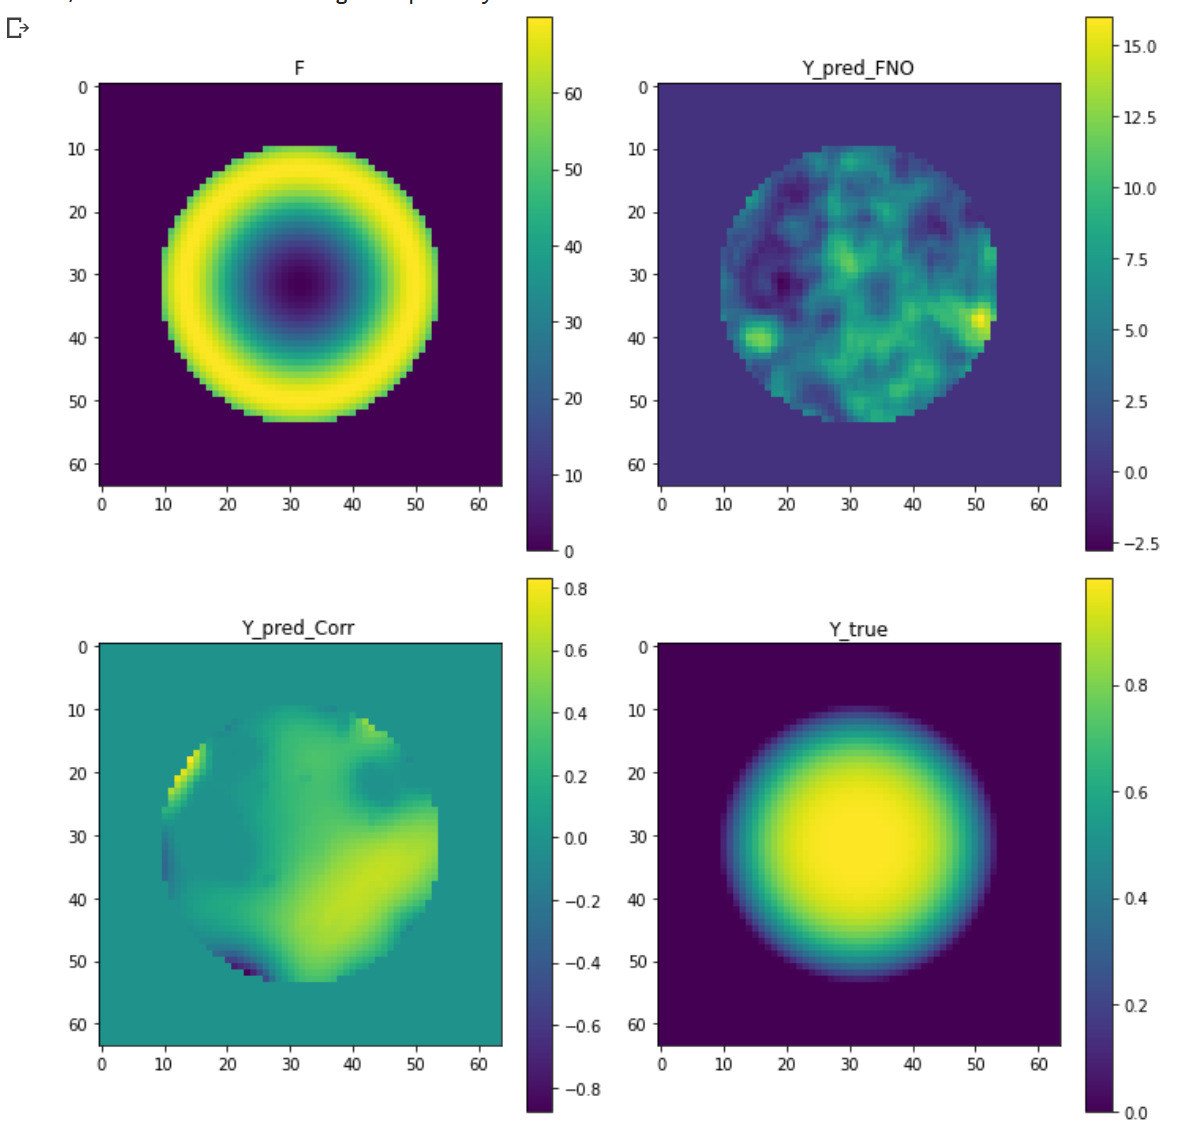
\includegraphics[width=0.45\linewidth]{resultats.png}
\end{minipage}

\begin{Rem}
	ERREUR : C'est logique !!! Le réseau n'a pas été entrainé pour ça ! (+ pb remarque d'avant.)
\end{Rem}




	
	\newpage 
	\section{Semaine 2 : 13/02/2023 - 17/02/2023}
\graphicspath{{semaines/semaine_2/images/}}

\begin{abstract}
	(Les résultats en semaine 1 ont été obtenus en début de semaine.)
	
	Après la semaine dernière, on s'est dit qu'une bonne idée serait de prendre une solution manufacturée (analytique) afin de pouvoir comparer les erreurs avec FEM classique, PhiFEM, le FNO et le FNO+correction. On a choisi de prendre $u$ comme une gaussienne et ainsi le f associé. Attention, il a fallut normaliser les F pour le FNO. On a également eut l'idée d'utiliser une solution sur-raffinée (à la place d'une solution exacte) mais ça n'a pas encore été testé.
\end{abstract}

\subsection{Génération de données}

On considère toujours $\Omega$ le cercle de rayon $\sqrt{2}/4$ et de centre $(0.5,0.5)$ avec $\Phi(x,y)=-1/8+(x-1/2)^2+(y-1/2)^2$ et le domaine fictif $O=(0,1)^2$ (\href{https://colab.research.google.com/drive/1Ymb1XZU80fwy7XxkL5_SsNs-ZVIVs3dm#scrollTo=GYtkSETwcBRp}{"DataGen\_PhiFEM\_u\_gaussienne"}).

On souhaite résoudre 
\begin{equation*}
	\begin{cases}
		-\Delta u &= f\,, \quad \text{dans $\Omega$}\,, \\
		u &= g\,, \quad \text{sur $\Gamma$}\,, \\
	\end{cases}
\end{equation*}

Notre solution analytique est
$$u_{ex}(x,y) = \exp\left(-\frac{(x-\mu_0)^2 + (y-\mu_1)^2}{2\sigma^2}\right)\,, $$ 
avec $\sigma \sim \mathcal{U}([0.1,0.6])$ et $\mu_0, \mu_1 \sim \mathcal{U}([-0.9, 0.9])$.

Ainsi 
$$f(x,y)=\left(\frac{2\sigma^2-(x-\mu_0)^2-(y-\mu_1)^2}{\sigma^4}\right)*\exp\left(-\frac{(x-\mu_0)^2 + (y-\mu_1)^2}{2\sigma^2}\right)$$
et
$$g(x,y)=u_{ex}(x,y)$$

Pour l'apprentissage du FNO, on va normaliser $f$ par $\max_f ||f||_{L^2(\Omega_h)}$

\textbf{Formulation faible :}

On utiliser une méthode directe pour inclure les conditions de Dirichlet homogène :

$$\int_{\Omega_h}\nabla(\bar{\phi}w)\nabla(\bar{\phi}v)-\int_{\partial\Omega_h}\frac{\partial}{\partial n}(\bar{\phi}w)\bar{\phi}v+G_h(w,v)=\int_{\Omega_h}f\bar{\phi}v-\left(\int_{\Omega_h}\nabla(g)\nabla(\bar{\phi}v)-\int_{\partial\Omega_h}\frac{\partial g}{\partial n}\bar{\phi}v\right)+G_h^{rhs}(v)$$
avec
$$G_h(w,v)=\sigma h\sum_{E\in\mathcal{F}_h^\Gamma}\int_E\left[\frac{\partial}{\partial n}(\bar{\phi}w)\right]\left[\frac{\partial}{\partial n}(\bar{\phi}v)\right]+\sigma h^2\sum_{T\in\mathcal{T}_h^\Gamma}\int_T \Delta(\bar{\phi}w)\Delta(\bar{\phi}v)$$
et
$$G_h^{rhs}(v)=-\sigma h^2\sum_{T\in\mathcal{T}_h^\Gamma}\int_T f\Delta(\bar{\phi}v)-\sigma h\sum_{E\in\mathcal{F}_h^\Gamma}\int_E\left[\frac{\partial g}{\partial n}\right]\left[\frac{\partial}{\partial n}(\bar{\phi}v)\right]-\sigma h^2\sum_{T\in\mathcal{T}_h^\Gamma}\int_T \Delta(g)\Delta(\bar{\phi}v)$$

\subsection{Résultat}

Voici un exemple de résultats obtenu sur $u$ une gaussienne (\href{https://colab.research.google.com/drive/1kcxNffAI2-fqmWv9swLnUrKGJRopedxF#scrollTo=oSFmuK2uVCXX}{"phifem\_u\_gaussienne"}).

\begin{minipage}{\linewidth}
	\centering
	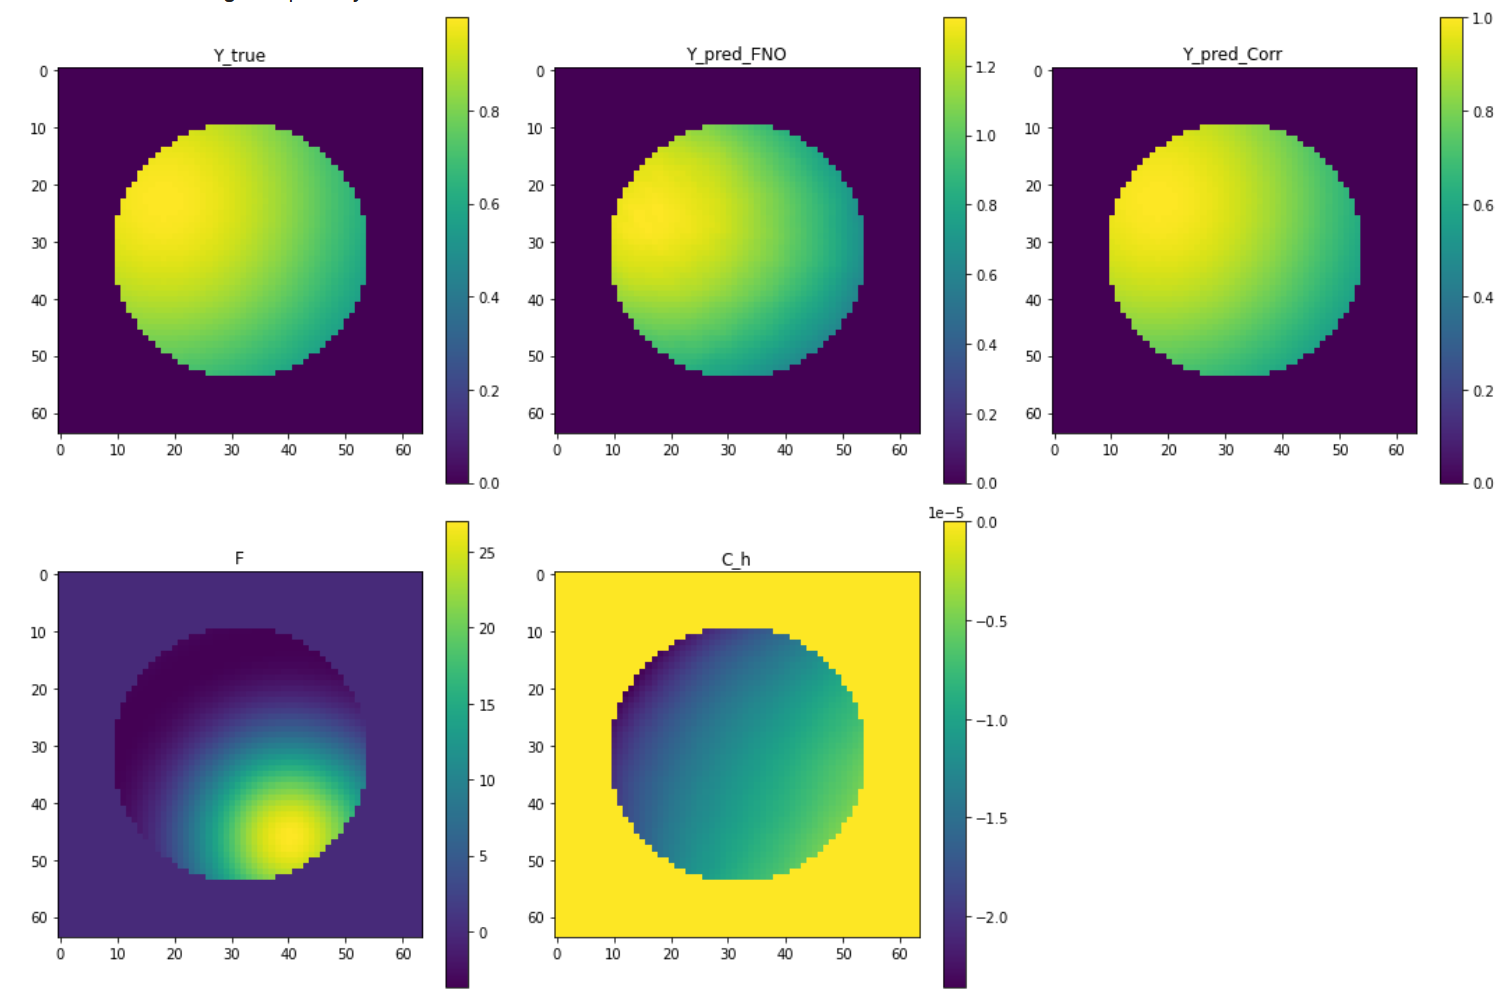
\includegraphics[width=0.45\linewidth]{resultat.png}
\end{minipage}

\conclusion{C'est en fin de semaine qu'on s'est rendue compte du problème du FNO : qu'il faut retourner $w$ et pas $u$. Les modifications ont été faites mais les résultats ne semblent toujours pas convaincant (résultats supprimés malencontreusement).
	
En fait, on a remarqué que prendre $g=u_{ex}$ sur $\Omega$ entier posait problème pour la correction, car on obtient $w=0$ et donc le problème de correction n'a plus de sens. Une solution à celà a été proposé par Emmanuel : il faudrait prendre $g=u_{ex}$ sur $\Gamma$ et étendre la solution (par exemple en utilisant un nouveau réseau de neurones qui nous fournirait une solution lisse). Mais pour l'instant, on va simplement choisir une autre solution analytique, où on n'est pas obligé de prendre $g=u_{ex}$ sur tout le domaine.

On a également eut l'idée de se ramener à un problème homogène (passage du problème en $f$ au problème en $\tilde{f}=f+\Delta g$)

Un autre problème constaté est qu'il faut utilisé le $\phi$ initial pour la génération des espaces $\mathcal{F}_h^\Gamma$ et $\mathcal{T}_h^\Gamma$.}
	
	\newpage
	\section{Semaine 3 : 20/02/2023 - 24/02/2023}
\graphicspath{{semaines/semaine_3/images/}}

\begin{abstract}
	Pour cette semaine, on considère une nouvelle solution analytique (solution trigonométrique : $\sin*\cos$). Avec cette nouvelle solution, on va pouvoir prendre g différent de $u_{ex}$ sur $\Omega$ comme souhaité pendant la semaine précédente. 
	
	A défaut de pouvoir faire tourner les entrainements (car plus d'units dispo sur colab) et en attente d'une solution avec v100, on va s'intéresser uniquement au problème de correction où on prendra comme $\bar{\phi}$ notre $u_{ex}$ ($-g$ si non homogène). En lui donnant comme nouvelle levelset notre solution exacte, $C$ doit être très proche de 1 (à l'erreur machine).  
\end{abstract}

\subsection{Génération des données}

On considère toujours $\Omega$ le cercle de rayon $\sqrt{2}/4$ et de centre $(0.5,0.5)$ avec $\Phi(x,y)=-1/8+(x-1/2)^2+(y-1/2)^2$ et le domaine fictif $O=(0,1)^2$.

On souhaite résoudre 
\begin{equation*}
	\begin{cases}
		-\Delta u &= f\,, \quad \text{dans $\Omega$}\,, \\
		u &= g\,, \quad \text{sur $\Gamma$}\,, \\
	\end{cases}
\end{equation*}

Notre solution analytique est
$$u_{ex}(x,y) = \frac{1}{\sin\left(k_1\frac{\pi}{2}\right)}\times\sin\left(k_1\frac{\pi}{2}\left(\frac{4}{\sqrt{2}}\right)^2\left((x-0.5)^2+(y-0.5)^2\right)\right)\times\cos(k_2(x^2+y^2))\,, $$ 

avec $k_1,k_2 \sim \mathcal{U}([0.1,0.5])$.

Ainsi 
$$g(x,y)=\cos(k_2(x^2+y^2))$$

On considérera également la solution analytique au problème homogène :
$$u_{ex}(x,y) = \frac{1}{\sin\left(k_1\frac{\pi}{2}\right)}\times\sin\left(k_1\frac{\pi}{2}\left(\frac{4}{\sqrt{2}}\right)^2\left((x-0.5)^2+(y-0.5)^2\right)\right)\times\cos\left(\frac{\pi}{2}\left(\frac{4}{\sqrt{2}}\right)^2\left((x-0.5)^2+(y-0.5)^2\right)\right)\,, $$ 

Les formulation faibles sont les mêmes que précédemment.

\subsection{Correction}

Dans un premier temps, on a pris notre nouvel levelset comme étant notre solution exacte sur une image 64*64 puis on interpoler cette levelset (\href{https://colab.research.google.com/drive/15rw2vTlf8yNBIuQPsFHzguUj5fmJiLf9#scrollTo=N2Z4fEjTNpAV}{"u\_trigo\_homogene"}). En prenant $\phi=u_{ex}$, on espère obtenir C très proche de 1 (en augmentant le degré d'interpolation, on espère atteindre l'erreur machine). Les résultats obtenus n'étaient pas bon :

\begin{minipage}{\linewidth}
	\centering
	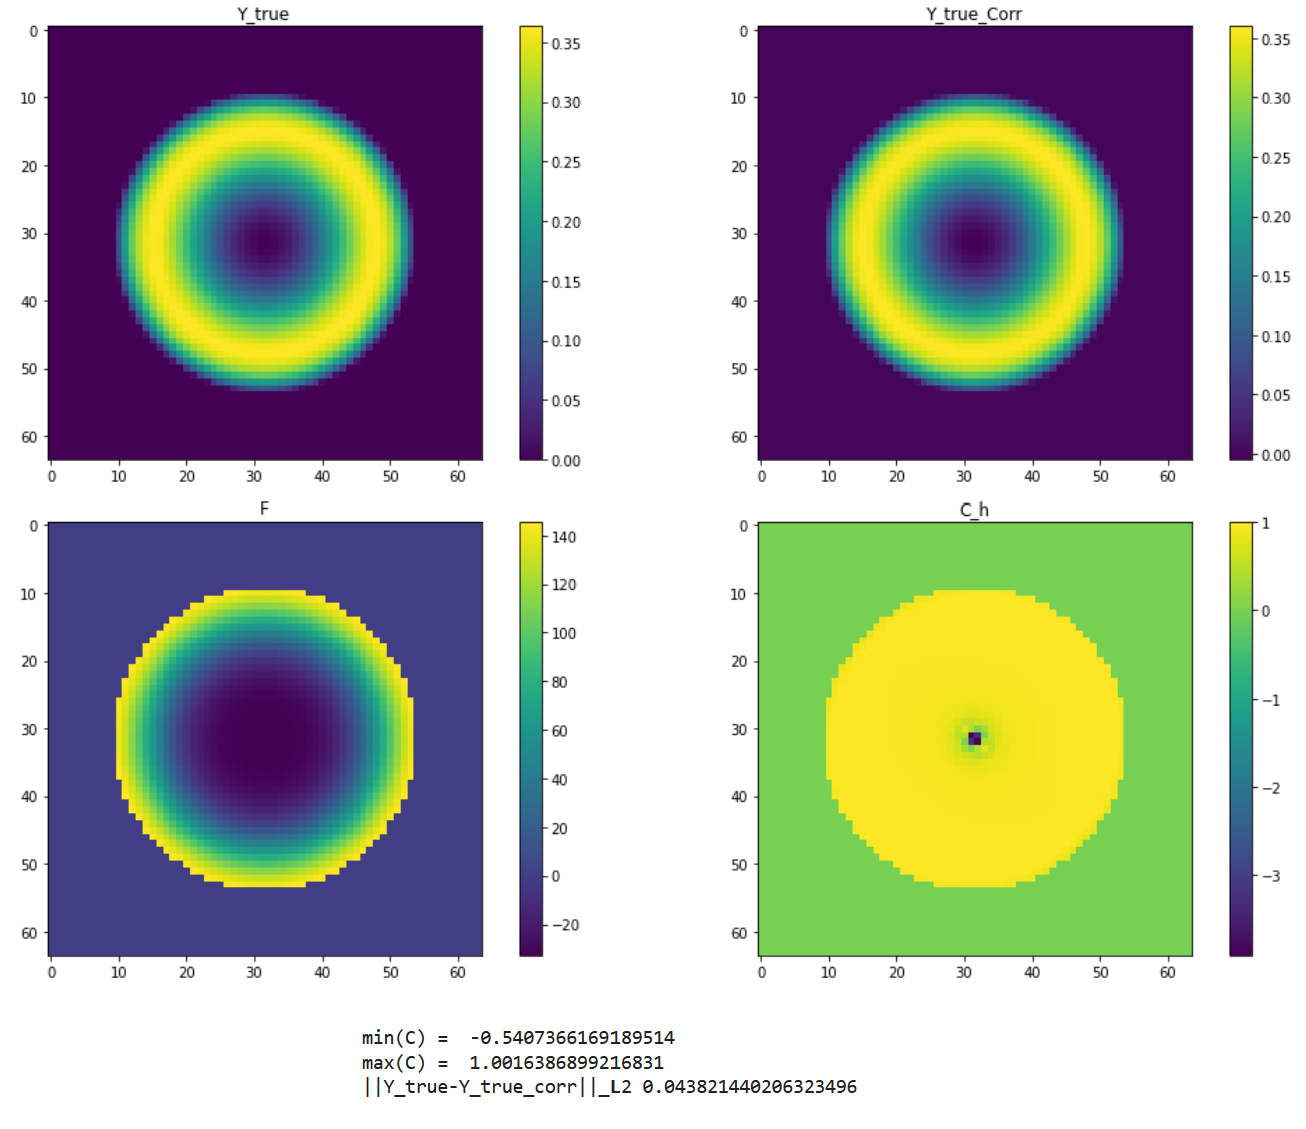
\includegraphics[width=0.45\linewidth]{resultats_correction.png}
\end{minipage}

\newpage 

En fin de semaine, on s'est rendue compte que l'interpolation de $\phi$ posait problème pour la correction. Lorsque $\bar{\phi}=u_{ex}$, on obtient bien l'erreur machine mais en lui donnant notre levelset sous la forme d'une image nb\_vert$\times$nb\_vert (ce qui est plus proche de ce que le réseau fournira), les résultats deviennent incohérents. On a donc tenter deux approches (\href{https://colab.research.google.com/drive/1JOC10OHCCNgTOCPD46bylKhlI1n1_bHR#scrollTo=0w0hQjVlLGwd}{"u\_trigo\_homogene\_modif"}): griddata (de scipy) et extrapolate (de FEniCS). L'option du extrapolate n'a pas fonctionné (nan ?). Pour l'autre option avec le griddata, on a constaté que interpoler avec tous les points de l'image était trop lourd, on a donc décidé de prendre pour chaque point (x,y) un certains nombres de points d'interpolations autour de lui. Voici les résultats obtenus avec différents nb\_vert et différents nombres de points d'interpolation :

\begin{minipage}{\linewidth}
	\centering
	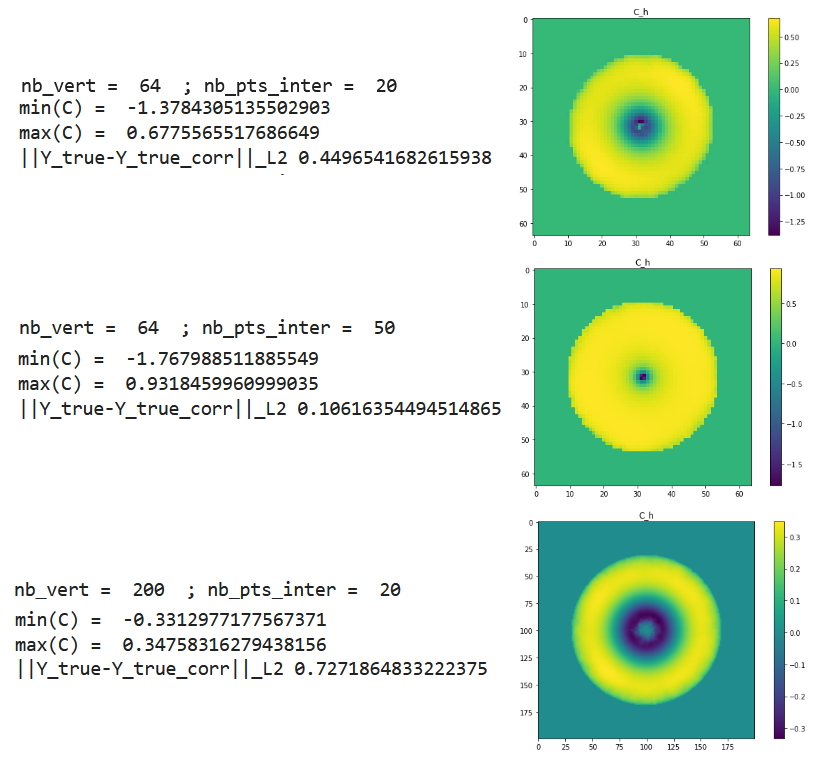
\includegraphics[width=0.6\linewidth]{griddata.png}
\end{minipage}

Ces résultats ont été obtenus la semaine suivante.


\conclusion{L'idée pour la semaine prochaine et d'effectuer quelques tests pour essayer de comprendre ce qui pose problème avec l'interpolation. Une fois ce type de problème réglé, on espère pouvoir entrainer le modèle sur la v100.}
	
	\newpage
	\section{Semaine 4 : 27/02/2023 - 03/03/2023}
\graphicspath{{semaines/semaine_4/images/}}

\begin{abstract}
	On cherche à comprendre les problèmes d'interpolation de phi dans le cadre de la correction sur la solution exacte du problème de poisson avec condition de dirichlet homogène. Après la réunion du 28/02 avec Emmanuel et Vanessa, les points suivants sont à traiter :
	\begin{enumerate}[label=\textbullet]
		\item tester avec solution analytique + perturbation !
		\item enlever les termes de stabilisation afin de voir si le problème est dans la dérivée seconde de phi
		\item visualiser le $\phi$ et le $\phi'$ EF et le comparer au $\phi$ et $\phi'$ analytique
		\item comprendre le problème du extrapolate
	\end{enumerate}
	Après la réception d'un ordinateur, on a passé la moitié de la semaine à essayer d'installer ce dont on avait besoin. En fin de semaine, les installations ont enfin été faite et je peux maintenant générer des données et entraîner le modèle sur ce nouveau PC.
\end{abstract}

\subsection{Génération des données}

On considère toujours $\Omega$ le cercle de rayon $\sqrt{2}/4$ et de centre $(0.5,0.5)$ avec $\Phi(x,y)=-1/8+(x-1/2)^2+(y-1/2)^2$ et le domaine fictif $O=(0,1)^2$.

On souhaite résoudre 
\begin{equation*}
	\begin{cases}
		-\Delta u &= f\,, \quad \text{dans $\Omega$}\,, \\
		u &= 0\,, \quad \text{sur $\Gamma$}\,, \\
	\end{cases}
\end{equation*}

Notre solution analytique est
$$u_{ex}(x,y) = \frac{1}{\sin\left(k_1\frac{\pi}{2}\right)}\times\sin\left(k_1\frac{\pi}{2}\left(\frac{4}{\sqrt{2}}\right)^2\left((x-0.5)^2+(y-0.5)^2\right)\right)\times\cos\left(\frac{\pi}{2}\left(\frac{4}{\sqrt{2}}\right)^2\left((x-0.5)^2+(y-0.5)^2\right)\right)\,, $$ 

avec $k_1 \sim \mathcal{U}([0.1,0.5])$.

\subsection{Correction}

On cherche à comprendre les problèmes d'interpolation de phi dans le cadre de la correction sur la solution exacte du problème de poisson avec condition de Dirichlet homogène (\href{https://colab.research.google.com/drive/17S0TrfstBv8vk6KR3uAy8gbeOcSkWPsY#scrollTo=7i8HL9-JKfEj}{"tests\_interpolation"}). On va effectuer plusieurs tests :

\subsubsection*{Solution analytique + Perturbation.}

Pour simuler la solution fournit par le FNO on va considérer comme nouvelle level-set notre solution analytique plus une petite perturbation. La perturbation choisie est définie par :
$$P(x,y)=\epsilon\times\sin(k_1(x+y))\times\cos(4\pi((x-0.5)^2+(y-0.5)^2))$$
On a alors
$$\Phi(x,y)=u_{ex}(x,y)+P(x,y)$$
En prenant $\epsilon=1$, on a :

\begin{minipage}{\linewidth}
	\centering
	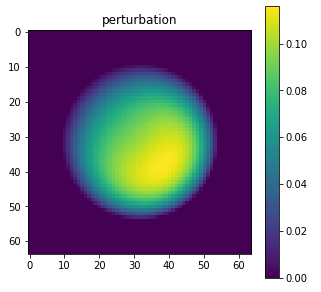
\includegraphics[width=0.3\linewidth]{perturbation.png}
\end{minipage}

On obtient en normes $L_2$ les différentes erreurs en fonction de $\epsilon=1e-k$ entre la solution initiale fournit $\Phi$ et le solution après correction $\Phi C$ : 

\begin{minipage}{\linewidth}
	\centering
	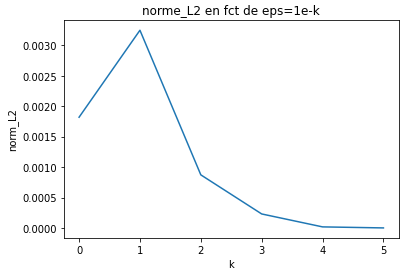
\includegraphics[width=0.45\linewidth]{erreurs_perturb.png}
\end{minipage}

Il semblerait que plus la perturbation est petite et plus l'erreur est petite. De plus, $C$ est de plus en plus proche de 1 :

\begin{minipage}{\linewidth}
	\centering
	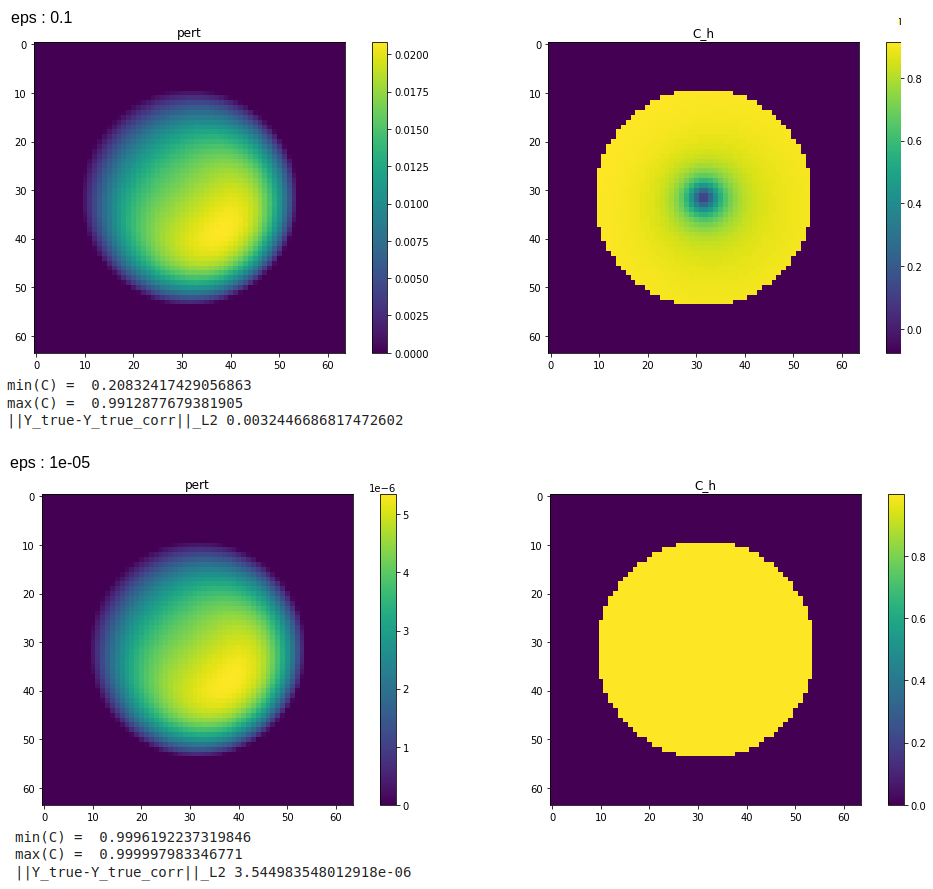
\includegraphics[width=0.55\linewidth]{results_perturb.png}
\end{minipage}

\subsubsection*{Griddata}

On a comparé $\Phi$ exact et notre $\Phi$ interpolé avec griddata (pour nb\_vert=64 et nb\_pts=20). Voici les résultats obtenus :

\begin{minipage}{\linewidth}
	\centering
	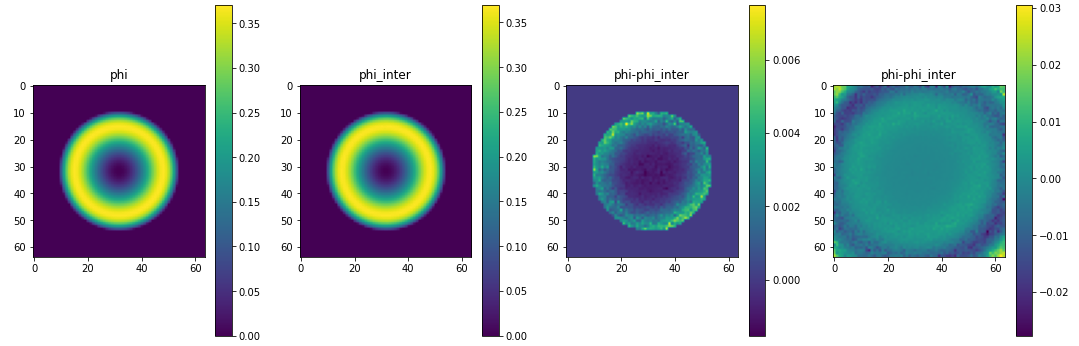
\includegraphics[width=0.9\linewidth]{results_griddata.png}
\end{minipage}

Il semblerait que sur le bord du cercle, les résultats soit moins bons. On a pas cherché à comprendre plus loin car on va utiliser la fonction extrapolate de FEniCS.


\subsubsection*{Extrapolate de FEniCS}

En milieu de semaine, on s'est rendu compte que le problème avec la foncion extrapolate que l'on avai eut la semaine dernière était que l'on pouvait n'incrémenter le degré d'interpolation que de 1.

\begin{minipage}{\linewidth}
	\centering
	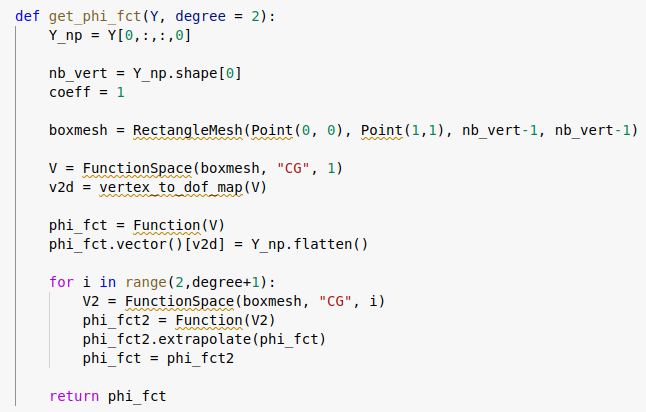
\includegraphics[width=0.5\linewidth]{get_phi_fct.png}
\end{minipage}

Voici les résultats obtenus pour une degré 2 :

\begin{minipage}{\linewidth}
	\centering
	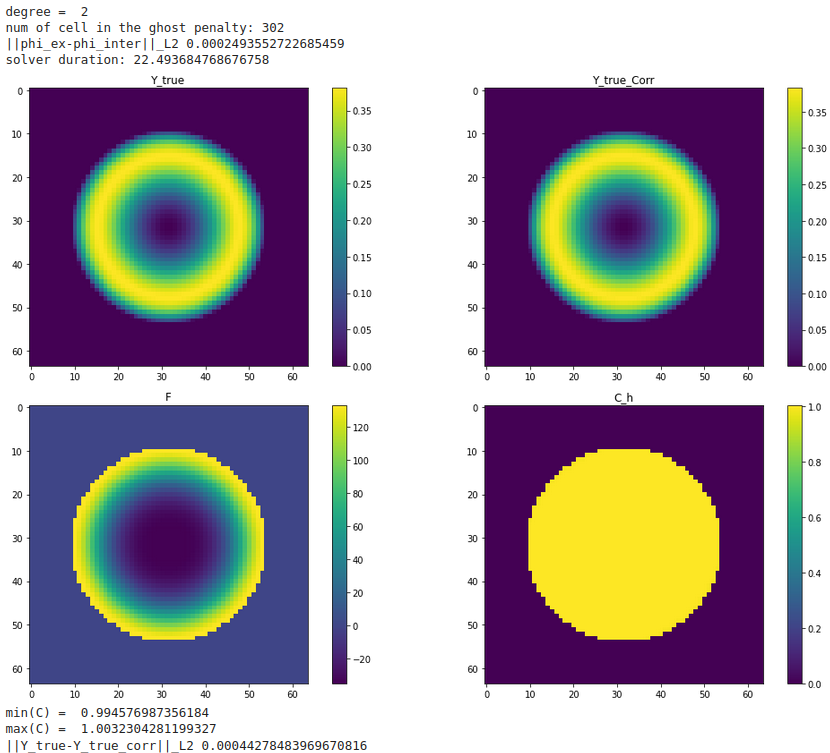
\includegraphics[width=0.9\linewidth]{results_extrapolate.png}
\end{minipage}


\conclusion{La semaine prochaine, on peut enfin entraîner le modèle car les installations ont été faites sur le nouveau pc.}

	
\end{document}